\documentclass[12pt, titlepage]{article}

\usepackage{fullpage}
\usepackage[round]{natbib}
\usepackage{multirow}
\usepackage{booktabs}
\usepackage{tabularx}
\usepackage{graphicx}
\usepackage{float}
\usepackage{hyperref}
\hypersetup{
    colorlinks,
    citecolor=blue,
    filecolor=black,
    linkcolor=red,
    urlcolor=blue
}

%% Comments

\usepackage{color}

\newif\ifcomments\commentstrue %displays comments
%\newif\ifcomments\commentsfalse %so that comments do not display

\ifcomments
\newcommand{\authornote}[3]{\textcolor{#1}{[#3 ---#2]}}
\newcommand{\todo}[1]{\textcolor{red}{[TODO: #1]}}
\else
\newcommand{\authornote}[3]{}
\newcommand{\todo}[1]{}
\fi

\newcommand{\wss}[1]{\authornote{blue}{SS}{#1}} 
\newcommand{\plt}[1]{\authornote{magenta}{TPLT}{#1}} %For explanation of the template
\newcommand{\an}[1]{\authornote{cyan}{Author}{#1}}

%% Common Parts

\newcommand{\progname}{ProgName} % PUT YOUR PROGRAM NAME HERE
\newcommand{\authname}{Team \#, Team Name
\\ Student 1 name
\\ Student 2 name
\\ Student 3 name
\\ Student 4 name} % AUTHOR NAMES                  

\usepackage{hyperref}
    \hypersetup{colorlinks=true, linkcolor=blue, citecolor=blue, filecolor=blue,
                urlcolor=blue, unicode=false}
    \urlstyle{same}
                                


\newcounter{acnum}
\newcommand{\actheacnum}{AC\theacnum}
\newcommand{\acref}[1]{AC\ref{#1}}

\newcounter{ucnum}
\newcommand{\uctheucnum}{UC\theucnum}
\newcommand{\uref}[1]{UC\ref{#1}}

\newcounter{mnum}
\newcommand{\mthemnum}{M\themnum}
\newcommand{\mref}[1]{M\ref{#1}}

\begin{document}

\title{Module Guide for \progname{}} 
\author{\authname}
\date{\today}

\maketitle

\pagenumbering{roman}

\section{Revision History}

\begin{tabularx}{\textwidth}{p{3cm}p{2cm}X}
\toprule {\bf Date} & {\bf Version} & {\bf Notes}\\
\midrule
Dec 23 & 1.0 & Module Decomp\\
Jan 3 & 1.1 & Added Type Modules\\
Jan 14 & 1.2 & Revised diagram to acknowledge Record Modules\\

\bottomrule
\end{tabularx}

\newpage

\section{Reference Material}

This section records information for easy reference.

\subsection{Abbreviations and Acronyms}

\renewcommand{\arraystretch}{1.2}
\begin{tabular}{l l} 
  \toprule		
  \textbf{symbol} & \textbf{description}\\
  \midrule 
  AC & Anticipated Change\\
  DAG & Directed Acyclic Graph \\
  M & Module \\
  MG & Module Guide \\
  OS & Operating System \\
  R & Requirement\\
  SC & Scientific Computing \\
  SRS & Software Requirements Specification\\
  \progname & Explanation of program name\\
  UC & Unlikely Change \\
  \wss{etc.} & \wss{...}\\
  \bottomrule
\end{tabular}\\

\newpage

\tableofcontents

\listoftables

\listoffigures

\newpage

\pagenumbering{arabic}

\section{Introduction}

Decomposing a system into modules is a commonly accepted approach to developing
software.  A module is a work assignment for a programmer or programming
team~\citep{ParnasEtAl1984}.  We advocate a decomposition
based on the principle of information hiding~\citep{Parnas1972a}.  This
principle supports design for change, because the ``secrets'' that each module
hides represent likely future changes.  Design for change is valuable in SC,
where modifications are frequent, especially during initial development as the
solution space is explored.  

Our design follows the rules layed out by \citet{ParnasEtAl1984}, as follows:
\begin{itemize}
\item System details that are likely to change independently should be the
  secrets of separate modules.
\item Each data structure is implemented in only one module.
\item Any other program that requires information stored in a module's data
  structures must obtain it by calling access programs belonging to that module.
\end{itemize}

After completing the first stage of the design, the Software Requirements
Specification (SRS), the Module Guide (MG) is developed~\citep{ParnasEtAl1984}. The MG
specifies the modular structure of the system and is intended to allow both
designers and maintainers to easily identify the parts of the software.  The
potential readers of this document are as follows:

\begin{itemize}
\item New project members: This document can be a guide for a new project member
  to easily understand the overall structure and quickly find the
  relevant modules they are searching for.
\item Maintainers: The hierarchical structure of the module guide improves the
  maintainers' understanding when they need to make changes to the system. It is
  important for a maintainer to update the relevant sections of the document
  after changes have been made.
\item Designers: Once the module guide has been written, it can be used to
  check for consistency, feasibility, and flexibility. Designers can verify the
  system in various ways, such as consistency among modules, feasibility of the
  decomposition, and flexibility of the design.
\end{itemize}

The rest of the document is organized as follows. Section
\ref{SecChange} lists the anticipated and unlikely changes of the software
requirements. Section \ref{SecMH} summarizes the module decomposition that
was constructed according to the likely changes. Section \ref{SecConnection}
specifies the connections between the software requirements and the
modules. Section \ref{SecMD} gives a detailed description of the
modules. Section \ref{SecTM} includes two traceability matrices. One checks
the completeness of the design against the requirements provided in the SRS. The
other shows the relation between anticipated changes and the modules. Section
\ref{SecUse} describes the use relation between modules.

\section{Anticipated and Unlikely Changes} \label{SecChange}

This section lists possible changes to the system. According to the likeliness
of the change, the possible changes are classified into two
categories. Anticipated changes are listed in Section \ref{SecAchange}, and
unlikely changes are listed in Section \ref{SecUchange}.

\subsection{Anticipated Changes} \label{SecAchange}

Anticipated changes are the source of the information that is to be hidden
inside the modules. Ideally, changing one of the anticipated changes will only
require changing the one module that hides the associated decision. The approach
adapted here is called design for
change.

\begin{description}
\item[\refstepcounter{acnum} \actheacnum \label{acEnhancedAuth}:] Enhanced Authentication Features.
\item[\refstepcounter{acnum} \actheacnum \label{acSessionUpdate}:] Session Management Updates.
\item[\refstepcounter{acnum} \actheacnum \label{acDbSchema}:] Database Schema Adjustments.
\item[\refstepcounter{acnum} \actheacnum \label{acUIEnhance}:] User Interface (UI) Enhancements.
\item[\refstepcounter{acnum} \actheacnum \label{acNewAlg}:] Integration of New Scheduling Algorithms.
\item[\refstepcounter{acnum} \actheacnum \label{acDataSecurity}:] Data Security and Privacy Updates.
\item[\refstepcounter{acnum} \actheacnum \label{acNotifSystem}:] Improved Notification System. 
\end{description}

\wss{Anticipated changes relate to changes that would be made in requirements,
design or implementation choices.  They are not related to changes that are made
at run-time, like the values of parameters.}

\subsection{Unlikely Changes} \label{SecUchange}

The module design should be as general as possible. However, a general system is
more complex. Sometimes this complexity is not necessary. Fixing some design
decisions at the system architecture stage can simplify the software design. If
these decision should later need to be changed, then many parts of the design
will potentially need to be modified. Hence, it is not intended that these
decisions will be changed.

\begin{description}
\item[\refstepcounter{ucnum} \uctheucnum \label{ucTechStack}:] Complete Redesign of the Technology Stack.
\item[\refstepcounter{ucnum} \uctheucnum \label{ucAuthFeatures}:] Elimination of Authentication Features.
\item[\refstepcounter{ucnum} \uctheucnum \label{ucDataStores}:] Replacement of Database Storage.
\item[\refstepcounter{ucnum} \uctheucnum \label{ucRBAC}:] Removal of Role-Based Access Control (RBAC).
\item[\refstepcounter{ucnum} \uctheucnum \label{ucSchedLogic}:] Simplification of Scheduling Logic.
\item[\refstepcounter{ucnum} \uctheucnum \label{ucEncryptStandard}:] Discontinuation of Encryption Standards.
\end{description}

\section{Module Hierarchy} \label{SecMH}

This section provides an overview of the module design. Modules are summarized
in a hierarchy decomposed by secrets in Table \ref{TblMH}. The modules listed
below, which are leaves in the hierarchy tree, are the modules that will
actually be implemented.

\begin{description}
\item [\refstepcounter{mnum} \mthemnum \label{mUI}:] User Interface Module
\item [\refstepcounter{mnum} \mthemnum \label{mAuth}:] Authentication Module
\item [\refstepcounter{mnum} \mthemnum \label{mTeamManagement}:] Team Management Module
\item [\refstepcounter{mnum} \mthemnum \label{mGameManagement}:] Game Management Module
\item [\refstepcounter{mnum} \mthemnum \label{mAnnouncements}:] Announcements Module
\item [\refstepcounter{mnum} \mthemnum \label{mStandings}:] Standings Module
\item [\refstepcounter{mnum} \mthemnum \label{mScheduling}:] Scheduling Module
\item [\refstepcounter{mnum} \mthemnum \label{mWaiver}:] Waiver Module
\item [\refstepcounter{mnum} \mthemnum \label{mPlayerT}:] PlayerT Module
\item [\refstepcounter{mnum} \mthemnum \label{mTeamT}:] TeamT Module
\item [\refstepcounter{mnum} \mthemnum \label{mGameT}:] GameT Module
\item [\refstepcounter{mnum} \mthemnum \label{mNotification}:] Notification Module
\item [\refstepcounter{mnum} \mthemnum \label{mBackend}:] Backend Module
\item [\refstepcounter{mnum} \mthemnum \label{mAlgo}:] Scheduling Algorithm Module
\item [\refstepcounter{mnum} \mthemnum \label{mGameslotT}:] GameslotT Module
\item [\refstepcounter{mnum} \mthemnum \label{mDivisionT}:] DivisonT Module
\item [\refstepcounter{mnum} \mthemnum \label{mStandingT}:] StandingT Module
\item [\refstepcounter{mnum} \mthemnum \label{mSeasonT}:] SeasonT Module
\item [\refstepcounter{mnum} \mthemnum \label{mRR}:] Reschedule Request Module


\end{description}


\begin{table}[h!]
\centering
\begin{tabular}{p{0.3\textwidth} p{0.6\textwidth}}
\toprule
\textbf{Level 1} & \textbf{Level 2}\\
\midrule

{Hardware-Hiding Module} & ~ \\
\midrule

\multirow{7}{0.3\textwidth}{Behaviour-Hiding Module} & User Interface Module\\
& Authentication Module\\
& Team Management Module\\
& Game Management Module\\
& Announcements Module\\
& Scheduling Module\\
& Standings Module\\
& Waiver Module\\
& PlayerT Module\\
& TeamT Module\\
& GameT Module\\
\midrule

\multirow{3}{0.3\textwidth}{Software Decision Module} & {Database Module}\\
& {Notification Module}\\
& {Scheduling Algorithm Module}\\
\bottomrule

\end{tabular}
\caption{Module Hierarchy}
\label{TblMH}
\end{table}

\section{Connection Between Requirements and Design} \label{SecConnection}

The design of the system is intended to satisfy the requirements developed in
the SRS. In this stage, the system is decomposed into modules. The connection
between requirements and modules is listed in Table~\ref{TblRT}.

\section{Module Decomposition} \label{SecMD}

Modules are decomposed according to the principle of ``information hiding''
proposed by \citet{ParnasEtAl1984}. The \emph{Secrets} field in a module
decomposition is a brief statement of the design decision hidden by the
module. The \emph{Services} field specifies \emph{what} the module will do
without documenting \emph{how} to do it. For each module, a suggestion for the
implementing software is given under the \emph{Implemented By} title. If the
entry is \emph{OS}, this means that the module is provided by the operating
system or by standard programming language libraries.  \emph{\progname{}} means the
module will be implemented by the \progname{} software.

Only the leaf modules in the hierarchy have to be implemented. If a dash
(\emph{--}) is shown, this means that the module is not a leaf and will not have
to be implemented.

\subsection{Behaviour-Hiding Module}

\subsubsection{User Interface Module (\mref{mUI})}

\begin{description}
\item[Secrets]: 
    \begin{itemize}
        \item The structure of inputs (e.g., username, password, team names, game scores, and scheduling information). 
        \item User interface components, logic, and states.
    \end{itemize}
    
\item[Services]: 
    \begin{itemize}
        \item Rendering views, collecting user input, and displaying data retrieved from the backend.
        \item Backend interactions to fetch data and send requests.
        \item Manages user role-based views.
    \end{itemize}

\item[Implemented By:] Team 6
    
\item[Type of Module:] Interface.

\end{description}

\subsubsection{Authentication Module (\mref{mAuth})}

\begin{description}
\item[Secrets:] The implementation details of password encryption, token generation, and user session management.

\item[Services:] Handles the following:
  \begin{itemize}
    \item User authentication, including login, registration, and logout.
    \item Verification of user credentials and assignment of roles (player, captain, administrator).
    \item Management of access tokens for secure API interactions.
  \end{itemize}

\item[Implemented By:] Team 6

\item[Type of Module:] Abstract Object
\end{description}

\subsubsection{Team Management Module (\mref{mTeamManagement})}

\begin{description}
\item[Secrets]: 
    \begin{itemize}
        \item Team creation for Captains and team joining joining processes and data for players.
        \item Waiver acceptance states and data.
    \end{itemize}
    
\item[Services]: 
    \begin{itemize}
        \item Handles captain input for team creation.
        \item Manages user-team associations (joining teams), and processing waiver sign-offs.
        \item Provides interface for captains to manage their teams (e.g., adding/removing players) and roster validation.
    \end{itemize}

\item[Implemented By:] Team 6
    
\item[Type of Module:] Abstract Object
\end{description}

\subsubsection{Game Management Module (\mref{mGameManagement})}

\begin{description}
  \item[Secrets] : 
  \begin{itemize}
      \item The structure of the input data includes game details (game ID, teams, scores, and status).
      \item Game record verification.
      \item Game statuses processes (e.g., scheduled, completed, canceled).
  \end{itemize}
  
\item[Services]: 
  \begin{itemize}
      \item Enables game score reporting and updating game statuses for appropriate roles.
      \item Updates store and retrieve game results to trigger standing updates.
  \end{itemize}
  \item[Implemented By:] Team 6
    
  \item[Type of Module:] Abstract Object
  \end{description}
\subsubsection{Announcements Module (\mref{mAnnouncements})}

\begin{description}
  \item[Secrets:] The structure of announcements, including title, message content, timestamps, as well as how announcements are stored, retrieved, and delivered to users, notifying them.

\item[Services]: 
  \begin{itemize}
      \item Allows admin to create, edit, and delete announcements for the league.
      \item Enables users to view announcements and ensures announcnement delivery via notifications.
  \end{itemize}

\item[Implemented By:] Team 6
    
\item[Type of Module:] Abstract Object
\end{description}
  
\subsubsection{Standings Module (\mref{mStandings})}

\begin{description}
  \item[Secrets:] The formulas for calculating rankings, win-loss records, and tie-breaking rules.
  
  \item[Services:] Handles the following:
    \begin{itemize}
      \item Tracks and updates league standings based on game results.
      \item Displays rankings, win-loss records, and statistical summaries for all teams.
      \item Supports tie-breaking scenarios and rankings by division.
    \end{itemize}
  
  \item[Implemented By:] Team 6
  
  \item[Type of Module:] Abstract Object
  \end{description}

  \subsubsection{Scheduling Module (\mref{mScheduling})}

  \begin{description}
    \item[Secrets:] Schedule management, including data structures and communication with the scheduling algorithm.
    
    \item[Services]: 
      \begin{itemize}
        \item Handles game schedule creation and updates.
        \item Manages scheduling constraints like team preferences.
        \item Integrates with the Scheduling Algorithm Module for optimization.
      \end{itemize}
    \item[Implemented By:] Team 6
    \item[Type of Module:] Abstract Object
    \end{description}

  \subsubsection{Waiver Module (\mref{mWaiver})}

  \begin{description}
    \item[Secrets:] Waiver completion data.
    \item[Services] :
      \begin{itemize}
        \item Manages waiver access and completion.
        \item Tracks waiver status for players.
        \item Integrates with user accounts to validate players.
      \end{itemize}
    \item[Implemented By:] Team 6
    \item[Type of Module:] Abstract Object
    \end{description}

  \subsubsection{PlayerT Module (\mref{mPlayerT})}

  \begin{description}
    \item[Secrets:] The data structure used to represent a player.
    \item[Services:] Holds the data of a player.
    \item[Implemented By:] Team 6
    \item[Type of Module:] Abstract Data Type
  \end{description}

  \subsubsection{TeamT Module (\mref{mTeamT})}

  \begin{description}
    \item[Secrets:] The data structure used to represent a team.
    \item[Services:] Holds the data of a team.
    \item[Implemented By:] Team 6
    \item[Type of Module:] Abstract Data Type
  \end{description}
    
  \subsubsection{GameT Module (\mref{mGameT})}

  \begin{description}
    \item[Secrets:] The data structure used to represent a game.
    \item[Services:] Holds the data of a game.
    \item[Implemented By:] Team 6
    \item[Type of Module:] Abstract Data Type
  \end{description}

  \subsubsection{GameslotT Module (\mref{mGameslotT})}

\begin{description}
  \item[Secrets:] The data structure used to represent a game slot.
  \item[Services:] Holds information about game time, field, date.
  \item[Implemented By:] Team 6
  \item[Type of Module:] Abstract Data Type
\end{description}

\subsubsection{DivisionT Module (\mref{mDivisionT})}

\begin{description}
  \item[Secrets:] The data structure used to represent a division.
  \item[Services:] Holds information about teams and standings within a division.
  \item[Implemented By:] Team 6
  \item[Type of Module:] Abstract Data Type
\end{description}

\subsubsection{StandingT Module (\mref{mStandingT})}

\begin{description}
  \item[Secrets:] The data structure used to represent a team's standings.
  \item[Services:] Tracks wins, losses, ties, and other metrics for ranking for playoffs.
  \item[Implemented By:] Team 6
  \item[Type of Module:] Abstract Data Type
\end{description}

\subsubsection{SeasonT Module (\mref{mSeasonT})}

\begin{description}
  \item[Secrets:] The data structure used to represent a season.
  \item[Services:] Holds information about teams, divisions, games, and timeframes for a season.
  \item[Implemented By:] Team 6
  \item[Type of Module:] Abstract Data Type
\end{description}

\subsubsection{Reschedule Request Module (\mref{mRR})}

\begin{description}
  \item[Secrets:] The data structure used to represent a reschedule request.
  \item[Services:] Allows for creating and tracking requests to reschedule games.
  \item[Implemented By:] Team 6
  \item[Type of Module:] Abstract Data Type
\end{description}


\subsection{Software Decision Module}

% \begin{description}
% \item[Secrets:] The design decision based on mathematical theorems, physical
%   facts, or programming considerations. The secrets of this module are
%   \emph{not} described in the SRS.
% \item[Services:] Includes data structure and algorithms used in the system that
%   do not provide direct interaction with the user. 
%   % Changes in these modules are more likely to be motivated by a desire to
%   % improve performance than by externally imposed changes.
% \item[Implemented By:] --
% \end{description}

\subsubsection{Notification Module (\mref{mNotification})}
\begin{description}
  \item[Secrets:] The protocols for sending important league updates via email notifications.
  \item[Services:] Sends notifications to users for important updates, such as schedule changes, game results, or captain messages.
  \item[Implemented By:] External Library
\end{description}



  \subsubsection{Backend Module (\mref{mBackend})}
  \begin{description}
    \item[Secrets:] The architecture, database schema, and integration logic for backend services.
    \item[Services]: 
      \begin{itemize}
        \item Manages server-side logic and handles API requests and responses.
        \item Database to storage and data retrieval (e.g., user data, schedules, game results, etc).
        \item Secure communication between the frontend and backend.
      \end{itemize}
    \item[Implemented By:] Team 6
  \end{description}

  \subsubsection{Scheduling Algorithm Module (\mref{mAlgo})}
  \begin{description}
    \item[Secrets:] The algorithm used to generate and optimize schedules, including constraints like team preferences, field availability, etc.
    \item[Services]:
      \begin{itemize}
        \item Generates game schedules based on team inputs and league constraints for admin use.
        \item Supports conflict resolution for rescheduling (e.g., double bookings, unavailable fields).
        \item Optimizes schedules to balance fairness and preferences across teams.
      \end{itemize}
    \item[Implemented By:] Team 6
  \end{description}
  
\section{Traceability Matrix} \label{SecTM}

This section shows two traceability matrices: between the modules and the
requirements and between the modules and the anticipated changes.

% the table should use mref, the requirements should be named, use something
% like fref
\begin{table}[H]
\centering
\begin{tabular}{p{0.2\textwidth} p{0.6\textwidth}}
\toprule
\textbf{Req.} & \textbf{Modules}\\
\midrule
R1 & \mref{mUI}, \mref{mAuth}, \mref{mBackend}\\
R2 & \mref{mUI}, \mref{mAuth}, \mref{mBackend}\\
R3 & \mref{mUI}, \mref{mScheduling}, \mref{mAlgo}\\
R4 & \mref{mUI}, \mref{mStandings}, \mref{mBackend}\\
R5 & \mref{mUI}, \mref{mTeamManagement}, \mref{mBackend}\\
R6 & \mref{mUI}, \mref{mTeamManagement}, \mref{mWaiver}, \mref{mBackend}\\
R7 & \mref{mUI}, \mref{mTeamManagement}, \mref{mScheduling}, \mref{mAlgo}, \mref{mBackend}\\
R8 & \mref{mUI}, \mref{mScheduling}, \mref{mAlgo}\\
R9 & \mref{mUI}, \mref{mAnnouncements}, \mref{mNotification}\\
R10 & \mref{mUI}, \mref{mScheduling}, \mref{mAlgo}\\
R10 & \mref{mUI}, \mref{mScheduling}, \mref{mAlgo}\\
R12 & \mref{mUI}, \mref{mGameManagement}, \mref{mBackend}\\
\bottomrule
\end{tabular}
\caption{Trace Between Requirements and Modules}
\textit{Note: The specific record modules are not included in traceability but are outlined in MIS.pdf}
\label{TblRT}
\end{table}

\begin{table}[H]
\centering
\begin{tabular}{p{0.2\textwidth} p{0.6\textwidth}}
\toprule
\textbf{AC} & \textbf{Modules}\\
\midrule
% \acref{acHardware} & \mref{mHH}\\
\acref{acEnhancedAuth} & \mref{mUI}, \mref{mAuth}, \mref{mBackend}\\
\acref{acSessionUpdate} & \mref{mUI}, \mref{mAuth}, \mref{mBackend}\\
\acref{acDbSchema} & \mref{mAuth}, \mref{mTeamManagement}, \mref{mStandings}, \mref{mBackend}\\
\acref{acUIEnhance} & \mref{mUI}, \mref{mNotification}\\
\acref{acNewAlg} & \mref{mScheduling}, \mref{mAlgo}\\
\acref{acDataSecurity} & \mref{mAuth}, \mref{mStandings}, \mref{mBackend}\\
\acref{acNotifSystem} & \mref{mNotification}, \mref{mBackend}\\
\bottomrule
\end{tabular}
\caption{Trace Between Anticipated Changes and Modules}
\label{TblACT}
\end{table}

\section{Use Hierarchy Between Modules} \label{SecUse}

In this section, the uses hierarchy between modules is
provided. \citet{Parnas1978} said of two programs A and B that A {\em uses} B if
correct execution of B may be necessary for A to complete the task described in
its specification. That is, A {\em uses} B if there exist situations in which
the correct functioning of A depends upon the availability of a correct
implementation of B.  Figure \ref{FigUH} illustrates the use relation between
the modules. It can be seen that the graph is a directed acyclic graph
(DAG). Each level of the hierarchy offers a testable and usable subset of the
system, and modules in the higher level of the hierarchy are essentially simpler
because they use modules from the lower levels.

\begin{figure}[H]
\centering
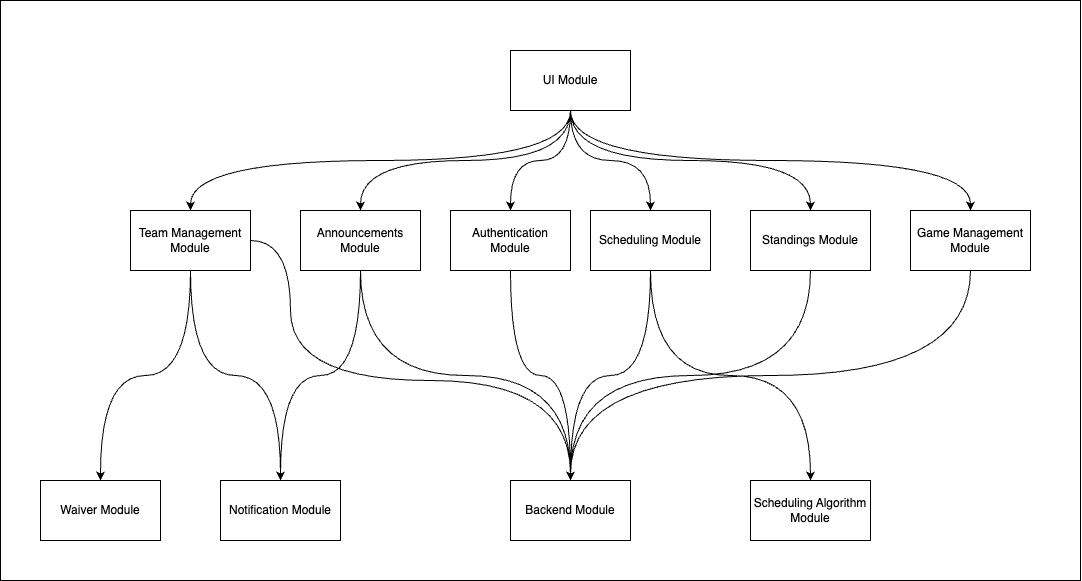
\includegraphics[width=1.1\textwidth]{module-decomp.png}
\caption{Use hierarchy among modules}
\textit{Note: Backend Module uses several record modules that represent data entities including Game, Type, Player, Season, Standing, Division, etc. The schemas for these record modules will be further specified in the MIS.pdf}
\label{FigUH}
\end{figure}

%\section*{References}

\section{User Interfaces}

\wss{Design of user interface for software and hardware.  Attach an appendix if
needed. Drawings, Sketches, Figma}

\section{Design of Communication Protocols}

\subsection*{Overview}
The communication protocols for the GSA Softball League platform are designed to ensure secure, reliable, and efficient interaction between system components and users. The platform employs a combination of RESTful APIs, web protocols, and encryption techniques to facilitate communication between the frontend, backend, and database, as well as external services.

\subsection*{Protocols}

\subsubsection*{Frontend to Backend Communication}
\begin{itemize}
    \item \textbf{Protocol}: HTTPS (Hypertext Transfer Protocol Secure)
    \item \textbf{Description}:
    \begin{itemize}
        \item All communication between the frontend and backend is secured using HTTPS, ensuring data integrity and confidentiality.
        \item RESTful APIs handle requests such as login, data retrieval, schedule updates, and notifications.
    \end{itemize}
    \item \textbf{Endpoints}:
    \begin{itemize}
        \item \texttt{/api/login}: Handles user authentication.
        \item \texttt{/api/schedule}: Retrieves game schedules.
        \item \texttt{/api/report}: Submits match results.
    \end{itemize}
\end{itemize}

\subsubsection*{Backend to Database Communication}
\begin{itemize}
    \item \textbf{Protocol}: MongoDB Wire Protocol (Over SSL/TLS)
    \item \textbf{Description}:
    \begin{itemize}
        \item Secure communication between the backend and the MongoDB database is facilitated by the MongoDB Wire Protocol over SSL/TLS.
        \item Queries include CRUD operations for users, teams, schedules, and standings.
    \end{itemize}
\end{itemize}

\subsubsection*{Backend to External Services}
\begin{itemize}
    \item \textbf{Protocol}: HTTPS with Third-Party APIs
    \item \textbf{Description}:
    \begin{itemize}
        \item External services such as email or SMS notifications (e.g., Twilio, SendGrid) communicate securely using HTTPS.
        \item APIs for notification services handle user alerts, such as schedule changes or reminders.
    \end{itemize}
\end{itemize}

\subsubsection*{Client to Client Communication}
\begin{itemize}
    \item \textbf{Protocol}: WebSockets (Optional)
    \item \textbf{Description}:
    \begin{itemize}
        \item Real-time updates for users, such as live score tracking or notifications, can be implemented using WebSocket connections.
    \end{itemize}
\end{itemize}

\subsubsection*{User Authentication Protocol}
\begin{itemize}
    \item \textbf{Protocol}: JWT (JSON Web Tokens) over HTTPS
    \item \textbf{Description}:
    \begin{itemize}
        \item Upon successful login, the backend issues a JWT to the client.
        \item JWTs are used to authenticate subsequent requests securely, reducing the need to reauthenticate for every action.
    \end{itemize}
\end{itemize}

\subsection*{Error Handling and Fault Tolerance}
\begin{itemize}
    \item \textbf{Timeouts}:
    \begin{itemize}
        \item API requests have a timeout of 30 seconds to avoid hanging requests.
        \item The frontend displays appropriate error messages if a timeout occurs.
    \end{itemize}
    \item \textbf{Retries}:
    \begin{itemize}
        \item Failed requests to external services are retried up to three times with exponential backoff.
    \end{itemize}
    \item \textbf{Error Codes}:
    \begin{itemize}
        \item Standardized HTTP status codes are used for API responses:
        \begin{itemize}
            \item \texttt{200}: Success
            \item \texttt{400}: Bad Request
            \item \texttt{401}: Unauthorized
            \item \texttt{403}: Forbidden
            \item \texttt{404}: Not Found
            \item \texttt{500}: Internal Server Error
        \end{itemize}
    \end{itemize}
\end{itemize}

\subsection*{Security Measures}
\begin{itemize}
    \item \textbf{Data Encryption}: All communication is encrypted using SSL/TLS to prevent data interception.
    \item \textbf{Authentication Tokens}: JWTs are signed and validated to ensure they are tamper-proof.
    \item \textbf{Input Validation}: All user inputs are validated to prevent injection attacks.
    \item \textbf{Access Control}: Role-based access control (RBAC) ensures that only authorized users can perform specific actions.
\end{itemize}

\wss{If appropriate}

\section{Timeline}

Note: Weeks 1 refers to the beginning of the year 2025

\subsection*{Phase 1: Documentation and Initial Setup (Week 1)}

\begin{enumerate}
    \item \textbf{Week 1: Finalization of Documentation}
    \begin{itemize}
        \item \textbf{Tasks}:
        \begin{itemize}
            \item Complete the \textbf{Module Interface Specification (MIS)}.
            \item Finalize the \textbf{Module Guide}.
            \item Create the initial sketches for the \textbf{User Interface.}
            \item Create the \textbf{Design of Communication Protocols}.
        \end{itemize}
        \item \textbf{Responsible Members}:
        \begin{itemize}
            \item \textbf{Damien Cheung:} Module Hierarchy, Module Decomposition, First Traceability Matrix, Use Hierarchy Between Modules,
            GameT Module, TeamT Module, PlayerT Module, Backend/Database Module.
            \item \textbf{Temituoyo Ugborogho:} Anticipated and Unlikely Changes, Second Traceability Matrix, Design of Communication Protocols,
            Timeline, Authentication Module.
            \item \textbf{Emma Wigglesworth:} User Interface, Scheduling Module, Scheduling Algorithm Module
            \item \textbf{Derek Li:} Notification Module, Announcement Module, Team Management Module, Waiver Module.
            \item \textbf{Jad Haytaoglu:} Game Management Module, User Interface Module.
            \item \textbf{All Members:} Review and finalization of documents.
        \end{itemize}
    \end{itemize}
\end{enumerate}

\subsection*{Phase 2: Core Module Development (Week 2)}

\begin{enumerate}
    \item \textbf{Week 2: Core Module Development}
    \begin{itemize}
        \item \textbf{Tasks}:
        \begin{itemize}
			\item Initialize and develop the \textbf{Database}.
            \item Develop the \textbf{Authentication Module} (login, session management, token generation).
            \item Create the \textbf{Scheduling Module} (game allocation logic).
            \item Implement the \textbf{Team Management Module} (team creation, roster management).
            \item Conduct preliminary unit testing for each core module.
        \end{itemize}
        \item \textbf{Responsible Members}:
        \begin{itemize}
			\item Damien Cheung and Jad Haytaoglu: Database.
            \item Temituoyo Ugborogho: Authentication Module.
            \item Emma Wigglesworth: Scheduling Module.
            \item Derek Li: Team Management Module.
        \end{itemize}
    \end{itemize}
\end{enumerate}

\subsection*{Phase 3: Supporting Module Development and Integration (Week 3)}

\begin{enumerate}
    \item \textbf{Week 3: Supporting Module Development and Integration}
    \begin{itemize}
        \item \textbf{Tasks}:
        \begin{itemize}
            \item Develop the \textbf{Notification Module} (alerts for schedule changes, announcements).
            \item Implement the \textbf{Game Management Module} (game data handling, score reporting).
            \item Build the \textbf{User Profile Module} (managing user preferences and settings).
            \item Integrate all developed modules (core and supporting) into a unified system.
            \item Conduct basic system-level integration tests.
        \end{itemize}
        \item \textbf{Responsible Members}:
        \begin{itemize}
            \item Derek Li: Notification Module Development.
            \item Jad Haytaoglu: Game Management Module and User Profile Module Development.
            \item Damien Cheung: Backend and Database Integration.
            \item All Members: Collaborative Integration Testing.
        \end{itemize}
    \end{itemize}
\end{enumerate}

\subsection*{Phase 4: System Testing and Final Refinements (Week 4)}

\begin{enumerate}
    \item \textbf{Week 4: System Testing and Final Refinements}
    \begin{itemize}
        \item \textbf{Tasks}:
        \begin{itemize}
            \item Conduct end-to-end system testing for all modules.
            \item Validate role-based access control (RBAC) functionality.
            \item Validate encryption protocols for secure data transfer (in transit and at rest).
            \item Prepare deployment documentation, including user guides and system setup instructions.
            \item Conduct a final review of traceability matrices and ensure alignment with anticipated changes.
        \end{itemize}
        \item \textbf{Responsible Members}:
        \begin{itemize}
            \item Damien Cheung and Jad Haytaoglu: Final Database and Backend Testing.
            \item Damien Cheung and Temituoyo Ugborogho: Final Communication Protocols and Traceability Documentation.
            \item Emma Wigglesworth, Temituoyo Ugborogho and Derek Li: Collaborative System Testing.
            \item All Members: Deployment Review.
        \end{itemize}
    \end{itemize}
\end{enumerate}

\subsection*{Key Details}
\begin{itemize}
    \item \textbf{Documentation}:
    \begin{itemize}
        \item Week 1 is entirely focused on finalizing all project documentation to ensure clarity and direction for subsequent development phases.
    \end{itemize}
    \item \textbf{Testing and Verification}:
    \begin{itemize}
        \item Unit testing will be performed for each module during development.
        \item Integration testing will be conducted immediately after module integration in \textbf{Week 3}.
        \item End-to-end testing will occur in \textbf{Week 4} to ensure Rev 0 readiness.
    \end{itemize}
\end{itemize}

\subsection*{Table of Responsibility To Date}

\begin{center}
	% \begin{tabular}{ | c | c | }
	\begin{tabular}{| p{0.3\textwidth} | p{0.6\textwidth} |}
		\hline
		Team Member & Responsibility \\ 
		\toprule

		\multirow{3}{0.3\textwidth}{Emma Wigglesworth}
		& User Interface \\
		& Scheduling Module \\
		& Scheduling Algorithm Module \\

		\midrule

		\multirow{4}{0.3\textwidth}{Derek Li}
		& Notification Module \\
		& Announcement Module \\
		& Team Management Module \\
		& Waiver Module \\

		\midrule

		\multirow{2}{0.3\textwidth}{Jad Haytaoglu}
		& Game Management Module \\
		& User Interface Module \\

		\midrule

		\multirow{8}{0.3\textwidth}{Damien Cheung}
		& Module Hierarchy \\
		& Module Decomposition \\
		& First Traceability Matrix \\
		& Use Hierarchy Between Modules \\
		& GameT Module \\
		& TeamT Module \\
		& PlayerT Module \\
		& Backend/Database Module \\

		\midrule

		\multirow{5}{0.3\textwidth}{Temituoyo Ugborogho}
		& Anticipated and Unlikely Changes \\
		& Second Traceability Matrix \\
		& Design of Communication Protocols \\
		& Timeline \\
		& Authentication Module \\

		\bottomrule

	\end{tabular}
\end{center}

More info can be found \href{https://github.com/dcheung11/team-6-capstone-project}{here.}

\wss{Schedule of tasks and who is responsible}

\wss{You can point to GitHub if this information is included there}

\bibliographystyle {plainnat}
\bibliography{../../../refs/References}

\newpage{}

\end{document}